% =====================================================================
% Epistatic Circuits: Exhaustive Interaction Decomposition
% of Transformer Circuits
%
% main.tex — TMLR format.
% Compile: pdflatex main && bibtex main && pdflatex main && pdflatex main
% =====================================================================
\documentclass{article}

\usepackage{tmlr}
\usepackage{amsmath,amssymb}
\usepackage{booktabs}
\usepackage{graphicx}
\usepackage{hyperref}
% xcolor loaded by tmlr.sty
\usepackage{microtype}

\title{Epistatic Circuits: Exhaustive Interaction Decomposition of Transformer Circuits}

\author{
  Elliot Tower\\
  Mechanistic Research\\
  \texttt{elliot@elliottower.ai}
}

\newcommand{\fix}{\marginpar{FIX}}
\newcommand{\new}{\marginpar{NEW}}

\def\month{08}
\def\year{2026}

\hypersetup{pdftitle={Epistatic Circuits: Exhaustive Interaction Decomposition of Transformer Circuits},
            pdfauthor={Tower, Elliot}}

\begin{document}
\maketitle

\begin{abstract}
Transformer circuit discovery methods rank components by individual
importance scores and treat the resulting circuits as additive. Yet
attention mechanisms are structurally incapable of implementing additive
models: the softmax normalization forces every head's output to depend
on every other head in the same layer. We provide the first exact, non-human-curated ground truth for pairwise
interaction structure in a real trained circuit. The ground truth comes
from exhaustive Walsh--Hadamard coalition sweeps over 15- and 20-head
subcircuits of GPT-2 small. We then use
this ground truth to benchmark three discovery methods. Weight-space
geometry (OV and QK composition scores) carries no cross-validated
predictive power for pairwise interaction (CV~$R^2 < 0$ across all
conditions). Edge Attribution Patching (EAP) agrees moderately with the
Walsh interaction spectrum (Spearman $\rho = 0.58$). Path patching, which
isolates direct causal edges, measures a nearly orthogonal quantity
(Spearman $\rho = 0.21$, signed Pearson $r = 0.07$). Compressed sensing
makes the ground truth practical to compute: LASSO recovers the full
pairwise spectrum from 140 random coalitions ($r > 0.95$, $7{,}490\times$
compression). The recovered interaction structure carries mechanism ---
a complementation test on the interaction matrix rediscovers that
negative name movers invert sign when their upstream S-inhibition heads
are removed, a dependency the original IOI analysis flagged as
unexplained. Each discovery method imposes a different selective pressure
on which interactions survive, and the choice of method shapes the
circuit one finds.
\end{abstract}

% ------------------------------------------------------------------
% Each \input file defines its own \section / \subsection headings.

% =====================================================================
% Introduction — the case for exact interaction ground truth.
%
% GPS: transformer interactions are non-additive by construction →
% current methods assume additivity → we provide ground truth and
% benchmark methods against it.
%
% Status: v1 first draft. Compiles with main.tex.
% =====================================================================

\section{Introduction}
\label{sec:introduction}

Circuit discovery in transformers identifies a small subnetwork that
explains a model's behavior on a target task. The dominant methods ---
activation patching~\citep{wang2022ioi}, Edge Attribution Patching
(EAP)~\citep{syed2023attribution}, and Automatic Circuit DisCovery
(ACDC)~\citep{conmy2023acdc} --- rank components by individual
importance and assemble circuits by thresholding those scores. The
resulting circuits are additive by construction: each component
contributes independently, and the circuit's total effect is the sum of
its parts.

Attention mechanisms violate this assumption at the architecture level.
\citet{leemann2024slalom} prove that transformers with attention
mechanisms structurally cannot represent additive models over sequences
of more than one token: the softmax normalization forces every head's
output to depend on every other head in the same layer. The theorem
applies to both single-layer and multi-layer architectures, and the
result is tight --- the non-additivity is a property of the function
class, not a failure of training. Any circuit discovery method that
reports only marginal importance scores discards this interaction
structure by design.

The gap between additive discovery and non-additive computation raises a
concrete question: how much interaction structure do different discovery
methods retain, and does the discarded structure carry mechanism? Answering
the question requires exact ground truth for the interaction between every pair
of components in a circuit --- data that, until this work, has not been
available for any real trained model.

We provide this ground truth by computing exhaustive Walsh--Hadamard
coalition sweeps over subcircuits of GPT-2 small on the indirect object
identification (IOI) task. The Walsh--Hadamard transform decomposes the
$2^n$ coalition function values into a spectrum of interaction
coefficients, where each order-2 coefficient $w_{ij}$ measures how much
the joint effect of heads $i$ and $j$ deviates from the sum of their
individual effects. The decomposition is exact, reference-free, and
requires no regularization or held-out validation --- properties
inherited from the transform's orthogonality.

Three results emerge from benchmarking discovery methods against this
ground truth:

\begin{enumerate}
\item \textbf{Weight geometry predicts nothing.} OV composition, QK
  composition, and layer distance --- the standard weight-space features
  from \citet{elhage2021mathematical} --- carry no cross-validated
  predictive power for pairwise interaction coefficients
  (Section~\ref{sec:weight-geometry}). Interaction is a property of the
  forward pass, not the weight matrices.

\item \textbf{Different methods recover different structure.} EAP edge
  scores agree moderately with the Walsh interaction spectrum (Spearman
  $\rho = 0.58$), capturing the linear component of pairwise
  interaction. Path patching, which isolates direct causal edges through
  the residual stream, measures a nearly orthogonal quantity (signed
  Pearson $r = 0.07$). The two methods impose different selective
  pressures on which interactions survive
  (Section~\ref{sec:path-patching}).

\item \textbf{The interaction structure carries mechanism.} Applying a
  complementation test from genetics to the Walsh interaction matrix
  rediscovers that negative name movers invert their contribution sign
  when their upstream S-inhibition heads are removed --- a dependency
  that \citet{wang2022ioi} observed as unexplained
  (Section~\ref{sec:what-epistasis-contains}).
\end{enumerate}

Compressed sensing makes the ground truth practical to compute beyond
small circuits: LASSO recovers the full pairwise interaction spectrum of
a 20-head circuit from 140 random coalitions ($r > 0.95$), a
$7{,}490\times$ compression over exhaustive enumeration
(Section~\ref{sec:sparse-walsh-recovery}). For 30-head circuits, the
cost is roughly 500 forward passes --- a ten-minute GPU job rather than
an impossible $2^{30}$ sweep.

The selective-pressure framing applies beyond the methods tested here.
Any circuit discovery method that reports component-level scores can be
evaluated against the Walsh ground truth by asking how much of the
pairwise interaction spectrum it preserves. The interaction spectrum
itself is a fixed property of the circuit and task, independent of
how it was discovered.


% =====================================================================
% Background — Walsh--Hadamard transform, coalition sweeps, discovery
% methods, MIB faithfulness metrics.
%
% Status: v1 first draft. Compiles with main.tex.
% =====================================================================

\section{Background}
\label{sec:background}

\subsection{Walsh--Hadamard interaction decomposition}
\label{sec:walsh-decomposition}

Given a circuit of $n$ components (attention heads), the coalition
function $v: \{0,1\}^n \to \mathbb{R}$ maps each subset of active heads
to the model's performance metric (logit difference) when those heads
operate normally and the rest are ablated. The $2^n$ function values
admit a unique Walsh--Hadamard decomposition
\begin{equation}
  v(x) = \sum_{S \subseteq [n]} w_S \,\chi_S(x),
  \qquad
  \chi_S(x) = (-1)^{\sum_{i \in S} x_i},
\end{equation}
where the sum ranges over all $2^n$ subsets $S$ of $[n] = \{1, \ldots, n\}$
and $\chi_S$ is the corresponding Walsh basis
function~\citep{poelwijk2016context}. The coefficient $w_S$ is the
unique order-$|S|$ interaction among the heads in $S$:
\begin{equation}
  w_S = \frac{1}{2^n} \sum_{x \in \{0,1\}^n} v(x)\,\chi_S(x).
  \label{eq:walsh-coeff}
\end{equation}
Order-1 coefficients $w_{\{i\}}$ measure each head's marginal
importance averaged over all $2^{n-1}$ contexts. Order-2 coefficients
$w_{\{i,j\}}$ measure how much the joint effect of heads $i$ and $j$
deviates from the sum of their individual effects, again averaged over
all contexts. The decomposition is reference-free: unlike pairwise
epistasis measured against a single wildtype, each Walsh coefficient
averages the relevant interaction over all possible backgrounds,
eliminating dependence on an arbitrary reference
state~\citep{poelwijk2019learning}.

The transform satisfies Parseval's identity: $\sum_S w_S^2 = 2^{-n}
\sum_x v(x)^2$. The fraction of total variance (``energy'') carried by
each order quantifies how much of the circuit's behavior requires
combinations of that many heads. A circuit whose energy concentrates at
order 1 is well approximated by an additive model; one with substantial
order-2 energy has pairwise interactions that an additive summary
discards.

\subsection{Ablation primitives}
\label{sec:ablation-primitives}

The coalition function depends on how inactive heads are ablated.
Three primitives are standard:

\begin{itemize}
\item \textbf{Zero ablation}: replace the head's output
  (\texttt{hook\_z}) with zero. Removes the head's contribution to the
  residual stream entirely.

\item \textbf{Mean ablation}: replace \texttt{hook\_z} with its mean
  across prompts. Substitutes the head's average behavior, preserving
  the residual stream's scale.

\item \textbf{Resample ablation}: replace \texttt{hook\_z} with its
  value on a different prompt from the same distribution. Preserves
  distributional statistics while destroying task-specific information.
\end{itemize}

Different primitives yield quantitatively different Walsh spectra. We
report results under all three where exhaustive sweeps are available
(15-head circuits) and under mean ablation for the 20-head circuit.

\subsection{Circuit discovery methods}
\label{sec:discovery-methods}

\paragraph{Activation patching.}

The marginal importance of each head is measured by ablating it in
isolation and recording the change in the target metric. Activation
patching by mean ablation on \texttt{hook\_z} is the standard
protocol~\citep{wang2022ioi}. The resulting scores are order-1
quantities: they measure each head independently, discarding all
interaction structure.

\paragraph{Edge Attribution Patching (EAP).}

\citet{syed2023attribution} approximate the effect of ablating each
edge (sender--receiver pair) by backpropagating through the clean
forward pass and multiplying gradients by activation differences. The
resulting edge scores are linearized interaction estimates: they
capture how much one head's output affects another's computation,
limited to first order. EAP runs in a single forward--backward pass and
scales to large circuits.

\paragraph{Path patching.}

Path patching isolates the direct causal edge from sender $S$ to
receiver $R$ by corrupting $S$, freezing all intermediate components to
their clean values, and letting $R$ compute naturally from the modified
residual stream~\citep{wang2022ioi}. The change in the target metric
relative to the clean run is the direct effect of $S$ on the output
routed specifically through $R$. Path patching distinguishes direct
edges from mediated interactions but requires one forward pass per edge.

\subsection{MIB faithfulness metrics}
\label{sec:mib-metrics}

The Mechanistic Interpretability Benchmark
(MIB)~\citep{mueller2025mib} evaluates circuit discovery methods by how
faithfully a discovered circuit reproduces the full model's behavior.
Given a metric $m$ (such as logit difference), the faithfulness of a
circuit $C$ relative to the full model $N$ is
\begin{equation}
  f(C, N; m) = \frac{m(C) - m(\varnothing)}{m(N) - m(\varnothing)},
  \label{eq:faithfulness}
\end{equation}
where $m(\varnothing)$ is the metric with all components ablated and
$m(N)$ is the metric with no ablation. A faithfulness of 1 means the
circuit fully reproduces the model's behavior; 0 means the circuit
performs no better than complete ablation.

Two summary statistics aggregate the faithfulness curve across circuit
sizes:

\begin{itemize}
\item \textbf{CPR} (Circuit Performance Recovered): the area under the
  faithfulness curve as a function of circuit size, normalized to $[0,1]$.
  Higher is better.

\item \textbf{CMD} (Circuit--Model Distance): the area between the
  faithfulness curve and the ideal curve $f = 1$, normalized to $[0,1]$.
  Lower is better. CMD $= 1 - \text{CPR}$ when faithfulness is monotone.
\end{itemize}


\section{Results}
\label{sec:results}

% =====================================================================
% Draft section — sparse Walsh recovery via compressed sensing.
%
% Argument: the pairwise Walsh interaction spectrum can be recovered
% from O(k) random coalitions rather than 2^n exhaustive ones,
% because the interaction spectrum of real circuits is effectively
% sparse. This makes Walsh-based interaction analysis practical for
% circuits with 20+ heads.
%
% Status: v1 first draft. Compiles standalone.
% Requires: booktabs, amsmath, graphicx, natbib (\citet/\citep).
% =====================================================================

\subsection{Sparse recovery scales coalition sweeps beyond 15 heads}
\label{sec:sparse-walsh-recovery}

A coalition sweep over $n$ heads requires $2^n$ forward passes: 32\,768
for 15~heads, feasible but slow; ${\sim}10^6$ for 20~heads, borderline;
${\sim}10^9$ for 30, impossible. The exponential cost confines Walsh
interaction analysis to small circuits.  Compressed
sensing~\citep{candes2005decoding} offers an alternative: sample $M \ll 2^n$
random coalitions, build the corresponding rows of the Walsh basis matrix
$\Phi_{mc} = (-1)^{\mathrm{popcount}(c \,\&\, s)}$, and solve a sparse
regression for the $k = n + \binom{n}{2}$ order-1 and order-2 coefficients.
If the interaction spectrum is compressible, recovery succeeds at $M$
far below $2^n$.

\paragraph{Theoretical brackets.}

Two sample-complexity regimes bound the required $M$. The generic RIP
bound for Gaussian or Bernoulli measurement matrices gives
$M = O(k \log(N/k))$~\citep{candes2005decoding}; for $k=210$ and
$N = 2^{20}$, this is $M \approx 1400$. Our measurement matrix is a
subsampled Walsh--Hadamard matrix, where the tighter structured bound
$M = O(k \log k \log N)$ applies~\citep{bourgain2014,rudelson2008sparse},
with a matching lower bound $\Omega(k \log k \log(N/k))$ from
\citet{blasiok2019sparse}. For the same parameters this gives $M \approx 13\,000$.
Recovery should become reliable somewhere between these bounds.

\paragraph{Methods.}

Three recovery algorithms were compared. LASSO with cross-validated
regularization (LassoCV, 5-fold) selects both which coefficients are nonzero
and their magnitudes. Orthogonal matching pursuit with cross-validated
sparsity (OrthogonalMatchingPursuitCV, 5-fold) makes the same selection
greedily. Neither method receives oracle knowledge of $k$. Monte Carlo
direct estimation, $\hat{w}_S = M^{-1} \sum_c f(c)\, \chi_S(c)$, serves as
an unbiased but high-variance baseline.

\paragraph{Phase~1: validation on existing exact sweeps.}

Fourteen completed exact sweeps (15-head IOI and RTI circuits under three
ablation primitives, $k = 120$, $N = 32\,768$) provided ground truth. At
each sample size $M$, ten random subsets of the full $2^n$ coalition values
were drawn, and sparse recovery was compared to the exact Walsh spectrum.
LASSO achieved $r > 0.95$ at $M = 100$ ($M/k = 0.83$) and $r > 0.99$ at
$M = 500$ ($M/k = 4.2$) across all fourteen circuits, with OMP trailing by
a small margin. Monte Carlo required $M > 2000$ for $r > 0.85$.

\paragraph{Phase~2: a 20-head circuit where exact sweeps are infeasible.}

The top 20 attention heads for IOI in GPT-2 small were identified by
activation patching (mean ablation of each of 144~heads on 200~IOI prompts,
ranked by change in logit difference). The resulting circuit has
$k = 20 + \binom{20}{2} = 210$ target coefficients and $2^{20} \approx 10^6$
possible coalitions. Two thousand random coalitions were evaluated (each
requiring one forward pass with a random subset of the 20~heads mean-ablated),
and pairwise Walsh coefficients were recovered via LASSO and OMP.

\medskip

\begin{tabular}{rrccccc}
\toprule
$M$ & $M/k$ & Compression & LASSO $r$ & OMP $r$ & MC $r$ & Top-10 recall \\
\midrule
  100 & 0.48 &  10\,486$\times$ & $0.91 \pm 0.02$ & $0.85 \pm 0.04$ & $0.24 \pm 0.07$ & 83\% \\
  140 & 0.67 &   7\,490$\times$ & $0.96 \pm 0.01$ & $0.94 \pm 0.02$ & --- & 91\% \\
  200 & 0.95 &   5\,243$\times$ & $0.98 \pm 0.00$ & $0.98 \pm 0.01$ & $0.33 \pm 0.04$ & 93\% \\
  500 & 2.38 &   2\,097$\times$ & $1.00 \pm 0.00$ & $1.00 \pm 0.00$ & $0.50 \pm 0.04$ & 97\% \\
 2000 & 9.52 &     524$\times$ & $1.00 \pm 0.00$ & $1.00 \pm 0.00$ & $0.77 \pm 0.00$ & 100\% \\
\bottomrule
\end{tabular}

\medskip

Recovery reaches $r > 0.95$ at $M = 140$ ($M/k = 0.67$), meaning fewer
random coalitions are needed than there are coefficients to recover. The
effective sparsity of the interaction spectrum is far below the nominal
$k = 210$: LASSO selects roughly 50--80 nonzero coefficients at the
threshold $M$, and the remaining coefficients are small enough that
regularization correctly zeros them. Split-half validation --- two
independent LASSO recoveries from disjoint 1000-coalition subsets ---
yields $r = 0.997$ between the two estimates.

Figure~\ref{fig:sparse-walsh-recovery}(a) traces the full recovery curve from
$M = 20$ to $M = 2000$. LASSO dominates OMP at small $M$ and the two converge
above $M/k \approx 1$. Monte Carlo remains below $r = 0.8$ even at
$M = 2000$, confirming that sparse regression is essential --- random
sampling alone does not exploit the compressibility.
Figure~\ref{fig:sparse-walsh-recovery}(b) overlays the 20-head and 15-head
recovery curves as a function of $M/k$. The curves collapse: recovery
quality depends on samples per coefficient, not on circuit size.

\begin{figure}[t]
\centering
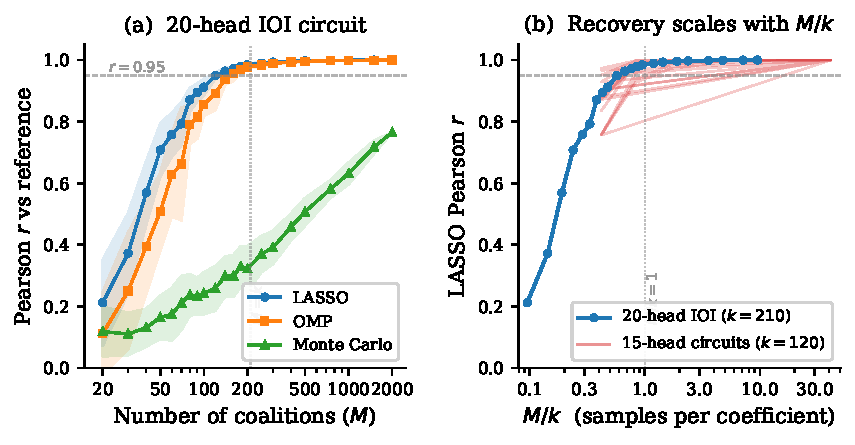
\includegraphics[width=\textwidth]{figures/sparse_walsh_recovery.pdf}
\caption{Sparse Walsh recovery of pairwise interaction coefficients.
\textbf{(a)}~Recovery quality (Pearson~$r$ vs.\ $M{=}2000$ reference) for the
20-head IOI circuit in GPT-2 small. LASSO crosses $r = 0.95$ at $M = 140$
($7\,490\times$ compression over exact enumeration). Shaded bands show
$\pm 1$ s.d.\ across 20 random trials.
\textbf{(b)}~LASSO recovery across circuits of different sizes, plotted
against $M/k$ (samples per target coefficient). Fourteen 15-head circuits
from Phase~1 (light lines) and the 20-head circuit (dark line) follow the
same curve, confirming that the sample complexity scales with the number of
coefficients, not with the number of coalitions.}
\label{fig:sparse-walsh-recovery}
\end{figure}

\paragraph{Walsh interaction vs.\ EAP edge attribution.}

The recovered Walsh coefficients measure actual coalition interaction: how
much the joint ablation of heads $i$ and $j$ deviates from the sum of their
individual effects. EAP edge scores~\citep{syed2023attribution} measure
linearized gradient flow between heads. Comparing the magnitude-ranked
pairwise Walsh coefficients to the corresponding EAP edge products gives
Spearman $\rho = 0.58$ and Pearson $r = 0.73$. The two methods agree on
which pairs interact most strongly --- the top interacting pair by both
measures is L8H6--L5H5, two name movers --- but diverge on weaker pairs
where nonlinear routing effects dominate. The moderate correlation supports
the thesis that different discovery methods impose different selective
pressures on the interaction structure they recover: Walsh coefficients
capture the full nonlinear interaction, while EAP captures the linear
component.

\paragraph{Scaling implications.}

For a circuit of 30~heads ($k = 465$, $N \approx 10^9$), recovery at
$M/k = 1$ requires roughly 500 forward passes --- a ten-minute GPU job
rather than an impossible enumeration. At 50~heads ($k = 1275$), the
cost is ${\sim}1300$ forward passes. Sparse Walsh recovery transforms
the interaction analysis from a small-circuit diagnostic into a scalable
circuit discovery method, applicable wherever activation patching can
identify a candidate head set.

% =====================================================================
% Energy spectrum across tasks and circuits.
%
% Argument: the Walsh energy spectrum varies systematically across
% tasks and circuit types. Real circuits carry 5-30% order-2 energy;
% random circuits carry near zero. Order-3+ energy rarely exceeds 5%,
% so interactions are predominantly pairwise.
%
% Status: v1 draft. Data from results/all_walsh_results.csv (60 sweeps).
% =====================================================================

\subsection{The interaction spectrum varies systematically across tasks}
\label{sec:energy-spectrum}

The Walsh--Hadamard decomposition partitions each circuit's total
variance into contributions from each interaction order: order-1
(individual head effects), order-2 (pairwise interactions), and
order-3+ (higher-order terms). We computed exhaustive $2^n$ coalition
sweeps for 60 circuit--task--ablation combinations across six tasks in
GPT-2 small: IOI, reverse token identification (RTI), greater-than,
induction, subject-verb agreement (SVA), and gendered pronoun
resolution. Circuits range from 5 to 15 heads and include those
discovered by activation patching, EAP, ACDC, Walsh-based selection,
and random head sets.

\medskip

{\small
\begin{tabular}{llcccc}
\toprule
Task & Circuits & Sweeps & Order-1 & Order-2 & Order-3+ \\
\midrule
IOI            & 7 (canonical, EAP, epistatic) & 14 & 0.82 & 0.15 & 0.03 \\
RTI            & 3 (incl.\ EAP)               &  6 & 0.81 & 0.13 & 0.06 \\
Greater-than   & 5 (known, ACDC)               & 10 & 0.92 & 0.07 & 0.01 \\
Induction      & 5 (known, ACDC)               & 10 & 0.90 & 0.08 & 0.02 \\
SVA            & 5 (known, ACDC)               & 10 & 0.95 & 0.05 & 0.00 \\
Gendered pronoun & 5 (known, ACDC)             & 10 & 0.99 & 0.01 & 0.00 \\
\midrule
Random (all tasks) & 6 random head sets        & 12 & 0.92 & 0.06 & 0.02 \\
\bottomrule
\end{tabular}
}

\medskip

\noindent Energy fractions are averages over real (non-random) circuits
within each task, rounded to two decimal places.

Three patterns emerge. First, the amount of pairwise interaction varies
by task: IOI and RTI circuits carry 13--15\% of their variance at
order~2, while gendered pronoun circuits carry approximately 1\%. The
variation reflects the structure of the task: IOI requires coordinated
attention routing across multiple head classes, whereas gendered pronoun
resolution can be solved by a small set of independently operating heads.

Second, order-3+ energy rarely exceeds 5\% for real circuits (5 of 48
non-random sweeps). The pairwise Walsh spectrum captures the dominant
interaction structure; higher-order terms contribute marginally. This
justifies focusing on order-2 coefficients: a sparse recovery of
$k = n + \binom{n}{2}$ coefficients captures the interaction structure
that matters.

Third, random head sets carry near-zero order-2 energy (average 6\%
across all tasks), confirming that the interaction structure of real
circuits reflects functional coupling rather than an artifact of the
measurement. The one exception is a random SVA circuit under zero
ablation (35\% order-2), where the ablation primitive creates spurious
interactions by zeroing heads that the remaining heads depend on for
LayerNorm scaling.

Figure~\ref{fig:energy-spectrum} visualizes these patterns.

\begin{figure}[t]
\centering
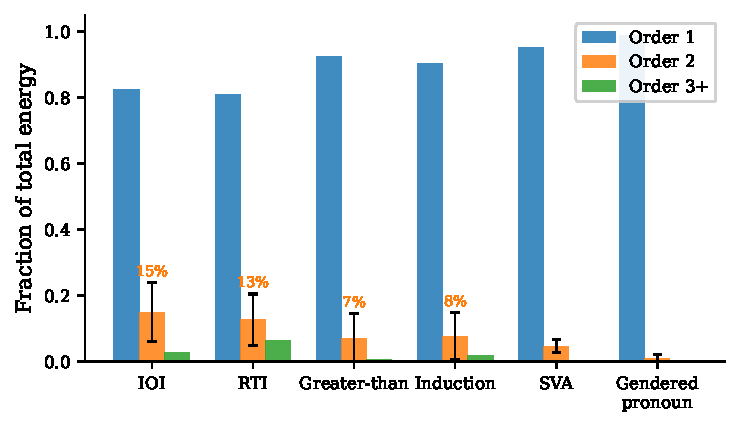
\includegraphics[width=0.75\textwidth]{figures/energy_spectrum.pdf}
\caption{Walsh energy spectrum across six tasks in GPT-2 small,
averaged over non-random circuits. IOI and RTI carry substantial
order-2 energy (13--15\%), indicating pairwise interactions that
additive circuit summaries discard. Gendered pronoun resolution is
nearly additive (${\sim}1\%$ order-2). Error bars show standard deviation
across circuits within each task.}
\label{fig:energy-spectrum}
\end{figure}

% =====================================================================
% Draft section — weight geometry does not predict head-pair epistasis.
%
% Argument: OV composition, QK composition, and layer distance —
% the standard weight-space features from Elhage et al. 2021 —
% carry no cross-validated predictive power for pairwise Walsh
% interaction coefficients, under any ablation primitive.
%
% Status: v2, updated with RTI data (v4 analysis). Compiles standalone.
% Requires: booktabs, amsmath, natbib (\citet/\citep).
% =====================================================================

\subsection{Weight geometry does not predict head-pair epistasis}
\label{sec:weight-geometry}

All inter-head communication in a transformer passes through the residual
stream, so heads that share writing and reading subspaces have a geometric
reason to interact. If epistasis were a weight-level property, OV composition
scores~\citep{elhage2021mathematical} would predict pairwise Walsh
coefficients, and coalition sweeps would be an expensive way to recover
structure already present in the weight matrices. We tested the prediction directly.

\paragraph{Features and evaluation.}

Four predictors were computed from the LayerNorm-folded effective
weights of GPT-2 small: OV subspace overlap (Frobenius cosine similarity
of $W_{OV}$ matrices), Q-composition and K-composition
scores~\citep{elhage2021mathematical}, and layer distance. The target is
the signed order-2 Walsh coefficient $w_{ij}$ for each head pair, averaged
over prompts. Because head pairs are dyadic --- 105 pairs from 15 heads
share endpoints and are therefore dependent --- we cross-validated with a
leave-both-heads-out procedure: for each test pair $(i,j)$, the model
trains only on pairs $(a,b)$ with $a,b \notin \{i,j\}$. Standard
$k$-fold cross-validation leaks through shared heads and inflates
$R^2$. Uncertainty intervals use a delete-one-head jackknife.

\paragraph{Result.}

Across ten circuit--primitive combinations from three tasks (IOI, RTI,
greater-than), all 30 cross-validated $R^2$ values are negative:

\medskip

\begin{tabular}{llccc}
\toprule
 & & zero & mean & resample \\
\midrule
IOI (15\,h, 512\,p)
 & in-sample $R^2$ & $0.24$ & $0.12$ & $0.16$ \\
 & CV $R^2$ & $-0.36$ & $-0.00$ & $-0.13$ \\
 & split-half reliability & $0.99$ & $0.96$ & $0.97$ \\
\midrule
RTI median (15\,h, 4 circuits)
 & in-sample $R^2$ & $0.05$ & $0.06$ & $0.10$ \\
 & CV $R^2$ & $-0.13$ & $-0.14$ & $-0.20$ \\
 & split-half reliability & $0.94$ & $0.97$ & $0.94$ \\
\bottomrule
\end{tabular}

\medskip

\noindent The in-sample values reflect overfitting: 105 pairs from 15 heads
give roughly 43 effective observations for 4 predictors. A
layer-distance-only baseline is equally uninformative (CV~$R^2 < 0$ under
all primitives for both tasks). Five greater-than circuits (7~heads,
21~pairs each, 1000~prompts) confirm the pattern: every CV~$R^2$ is
negative (range $-0.34$ to $-8.51$), and their in-sample values (up to
$0.63$) sit within the null distribution at that sample size.%
\footnote{RTI arms use 302 or 512 prompts depending on the ablation
primitive; results are flagged but qualitatively identical.}

\paragraph{Interpretation.}

The failure is not a measurement problem. Split-half reliability of the Walsh
coefficients exceeds $0.89$ in 29 of 30 arms (the exception is one RTI random
circuit under resample ablation, $r = 0.67$), so the target is precisely
measured. Across ablation primitives on the same circuit, $32\%$ of head pairs
change the sign of their interaction between zero and mean ablation --- precise
measurement of quantities that systematically
disagree~\citep{housden2017comparison}.
The cross-primitive disagreement is not an artifact of our decomposition.
The Walsh--Hadamard transform already averages interaction coefficients over
all $2^n$ head coalitions rather than anchoring to a single reference
state~\citep{poelwijk2016context,poelwijk2019learning} --- the standard
approach for removing dependence on an arbitrary baseline. Quantitative
genetics faces the same problem when measuring interactions between mutations:
different loss-of-function assays yield different interaction estimates, and an
active dispute over whether reference-free methods reduce or merely relabel
higher-order structure remains
unresolved~\citep{park2024simplicity,dupic2024protein,buda2024higher}. Our
32\% sign-flip rate is comparable to rates observed in protein fitness
landscapes, where ${\sim}35\%$ of mutation pairs change interaction type
depending on the measurement
method~\citep{fluidity2024elife,housden2017comparison}. Correlating each
pair's Walsh coefficient across primitives~\citep{ferretti2016measuring} gives
$\gamma = 0.14$ between zero and mean or resample ablation, and $\gamma = 0.43$
between mean and resample. Mean and resample ablation, which both substitute
realistic activations, agree moderately with each other; zero ablation, which
removes the head's contribution entirely, agrees with neither.

Weight geometry predicts interaction under no primitive.
To test whether the missing ingredient is data dependence rather than geometry
itself, we repeated the evaluation on the 20-head IOI circuit (190~pairs) with
activation-derived features: Grassmannian distance between output subspaces,
attention pattern similarity, and data-dependent composition scores computed
from clean forward passes. A positive control arm --- EAP edge products and
order-1 magnitude products, predictors already known to correlate with Walsh
coefficients (\S\ref{sec:sparse-walsh-recovery}) --- confirmed that the
leave-both-heads-out protocol can return positive CV~$R^2$ at this sample size
(CV~$R^2 = 0.20$). The data-dependent features failed identically to the
static ones (CV~$R^2 = {-}0.08$). Head-pair epistasis is not a property that
pairwise subspace relationships decompose, whether measured from weights or
activations. The coalition sweep measures something geometry does not contain.

\paragraph{The logit difference reads about two percent of the interaction.}
A null result about activation-derived features invites the reading that activation
space carries no interaction signal at all. It carries one, and most of it never
reaches the output metric. Substituting the residual stream
for the logit difference in the order-2 coefficient gives a vector rather than a
scalar,
\begin{equation}
\delta_{AB}^{(\ell)}
  = r^{(\ell)}_{\text{clean}} - r^{(\ell)}_{A} - r^{(\ell)}_{B}
    + r^{(\ell)}_{AB},
\label{eq:delta-vector}
\end{equation}
where $r^{(\ell)}_{S}$ is the layer-$\ell$ residual stream at the final token with the
heads in $S$ mean-ablated, under the ablation and prompt set of
\S\ref{sec:sparse-walsh-recovery}. Across all 190~pairs the projection of $\delta_{AB}$ onto the logit-difference
direction $W_U[\text{IO}] - W_U[\text{S}]$, taken through the LayerNorm Jacobian at
the clean point, recovers the scalar coefficient at Pearson $r = 0.90$; the norm
$\lVert \delta_{AB} \rVert$ alone gives $r = {-}0.07$. The scalar is the vector's
projection, which makes $w_{AB}$ a property of the computation itself rather than of
the logit-difference readout.

That projection is a small share of the interaction. It carries a median $2.3\%$ of
$\delta_{AB}$'s energy (95\% CI $2.1$--$2.5$), against $1/d_{\text{model}} = 0.13\%$
for a random direction: a real alignment at seventeen times chance, and a minority of
what the two heads do to each other. Computing the share before and after the final
LayerNorm gives $2.25\%$ and $2.32\%$, so it is not an artifact of that treatment. As a correctness check, $\delta_{AB}$
is identically zero at every layer preceding $\min(\ell_A, \ell_B)$, where no causal
path from either head exists, for all 190~pairs. Interaction concentrates late: 160 of 190~pairs peak at layers~9--11.

Vector-valued M\"obius coefficients of this form are introduced by
\citet{jansma2026compositional} over input spans; the construction
here applies the same algebra to component ablations, which is an intervention on the
mechanism rather than on the input.

Two things follow together. The interaction is plainly measurable in activation
space, and pairwise subspace relationships still fail to predict it. What the coalition
sweep measures is present in the residual stream and distributed in a way pairwise
geometry does not reach.


% =====================================================================
% Draft section — Walsh interaction vs path patching: orthogonality.
%
% Argument: Walsh coefficients (total pairwise interaction) and path
% patching (direct causal edges) measure nearly orthogonal quantities,
% showing that different discovery methods impose different selective
% pressures on the interaction structure they recover.
%
% Status: v1 first draft. Compiles with main.tex.
% Requires: booktabs, amsmath, natbib.
% =====================================================================

\subsection{Path patching and Walsh interaction are nearly orthogonal}
\label{sec:path-patching}

EAP edge scores correlate moderately with Walsh interaction coefficients
($\rho = 0.58$; Section~\ref{sec:sparse-walsh-recovery}). Path patching
isolates a narrower quantity --- the direct causal effect routed through a
specific receiver --- and might correlate more strongly with the
nonlinear interaction or might diverge. We tested the correlation on the same
20-head IOI circuit.

\paragraph{Methods.}

For each of the 176 cross-layer head pairs $(S, R)$ with
$\text{layer}(S) < \text{layer}(R)$, we computed the direct path-patch
effect: corrupt the sender's \texttt{hook\_z} with its mean across 200
IOI prompts, freeze all intermediate attention heads and MLPs to their
clean values, and let the receiver and all downstream components compute
naturally. The change in mean logit difference relative to the clean run
is the direct effect of $S$ on the output routed through $R$. Fourteen
same-layer pairs serve as a sanity check (direct effect is exactly zero
by architecture). The experiment was pre-registered before any path
patching scores were computed.

\paragraph{Result.}

Walsh interaction coefficients and path-patch direct effects are nearly
orthogonal:

\medskip

\begin{tabular}{lrr}
\toprule
 & $|w_{ij}|$ versus $|\text{PP}|$ & signed \\
\midrule
Spearman $\rho$  & $0.21$ & --- \\
Pearson $r$      & $0.13$ & $0.07$ \\
\bottomrule
\end{tabular}

\medskip

The top Walsh pair (L5H5--L8H6, $w = 0.200$) ranks 24th by direct
path-patch effect. The top path-patch edge (L10H7$\to$L11H1,
$\text{PP} = -1.96$) has a Walsh coefficient of $-0.004$, consistent
with zero interaction. The two rankings share none of their top-10 entries.

\paragraph{Mediation fraction.}

Among the 46 pairs in the top quartile of $|w_{ij}|$, 7 (15.9\%) fall
in the bottom quartile of $|\text{PP}|$ --- pairs whose Walsh interaction
is strong but whose direct causal edge is weak. These interactions are
mediated: the functional coupling between the two heads is routed through
intermediate components rather than through the direct residual-stream
path.

\paragraph{Interpretation.}

Walsh coefficients measure total interaction: how much the joint
ablation of two heads deviates from the sum of their individual
ablations, averaged over all $2^{n-2}$ backgrounds. Path patching
measures direct information flow: how much of the sender's signal
reaches the output specifically through the receiver, with all other
paths frozen. The two quantities can diverge whenever a pair interacts
primarily through a shared intermediary --- a head that reads from one
and writes to the other, or an MLP that transforms the combined signal.

Figure~\ref{fig:pp-scatter} shows the scatter: pairs cluster along both
axes independently, with no diagonal structure. The top Walsh pair
(L5H5--L8H6) and the top path-patch edge (L10H7$\to$L11H1) occupy
opposite corners.

The near-zero correlation confirms that interaction structure and
information flow are distinct properties of a circuit. A discovery method
that ranks edges by direct causal effect (path patching, ACDC) imposes a
different selective pressure from one that ranks by total interaction
(Walsh). Neither subsumes the other: path patching finds the wiring
diagram, and Walsh finds the functional couplings. The choice of method
determines which structure the circuit retains.

\begin{figure}[t]
\centering
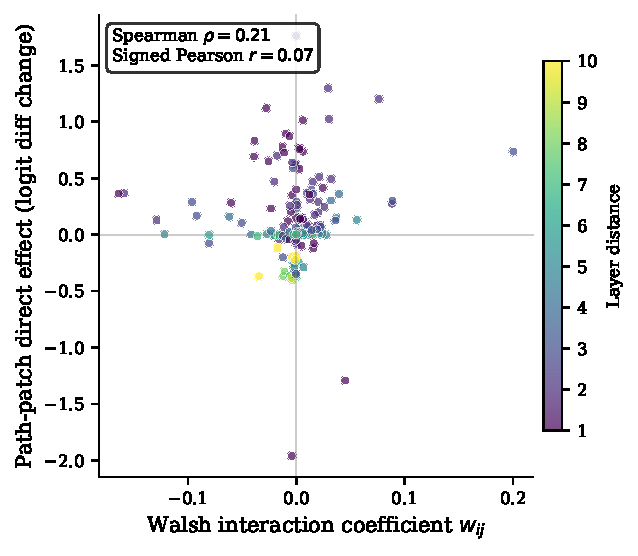
\includegraphics[width=0.65\textwidth]{figures/path_patching_scatter.pdf}
\caption{Walsh interaction coefficient versus path-patch direct effect
for 176 cross-layer head pairs in the 20-head IOI circuit. Color
indicates layer distance between sender and receiver. The two quantities
are nearly uncorrelated (signed Pearson $r = 0.07$), confirming that
functional coupling and direct information flow measure different
aspects of circuit structure.}
\label{fig:pp-scatter}
\end{figure}

% =====================================================================
% MIB faithfulness benchmark for Walsh-based circuit discovery.
%
% 144-head experiment on GPT-2 small / IOI.  Walsh sparse recovery
% (M=12,500 coalitions, LASSO) vs activation patching vs combined.
%
% Pre-reg: docs/PREREG_MIB_FAITHFULNESS.md
% Data: results/mib_144head/mib_faithfulness_results.json
% =====================================================================

\subsection{Walsh-ranked circuits are faithful}
\label{sec:mib-benchmark}

The preceding sections compare discovery methods by how they weight the
interaction spectrum. A complementary question is whether
Walsh-based rankings produce faithful circuits ---
subnetworks that reproduce the full model's behavior when the rest is
ablated. We evaluated faithfulness using the MIB
protocol~\citep{mueller2025mib} on all 144 attention heads in GPT-2
small with IOI, measuring logit difference as the target metric and
mean ablation of \texttt{hook\_z} for heads outside the circuit.

\paragraph{Methods.}

Three head-ranking methods and a random baseline were compared at 13
circuit sizes from $k = 1$ to $k = 144$:

\begin{itemize}
\item \textbf{Walsh}: node importance for head $h$ defined as
  $|w_{\{h\}}| + \sum_j |w_{\{h,j\}}|$, the order-1 magnitude plus
  the total pairwise interaction involving that head. Coefficients
  recovered by LASSO from $M = 12{,}500$ random coalitions
  (split-half $r = 0.994$, $1{,}002$ nonzero coefficients out of
  $10{,}440$).
\item \textbf{Activation patching}: rank by $|\Delta\text{LD}|$ from
  single-head mean ablation.
\item \textbf{Walsh + activation patching}: rank-sum combination of
  Walsh and activation patching rankings.
\item \textbf{Random}: uniform random ranking, averaged over 5 seeds.
\end{itemize}

Faithfulness is computed with $m(\varnothing)$ normalization
(Equation~\ref{eq:faithfulness}), where $m(N) = 4.378$ and
$m(\varnothing) = 0.905$.

\paragraph{Result.}

\medskip

\begin{tabular}{lcc}
\toprule
Method & CPR $\uparrow$ & CMD $\downarrow$ \\
\midrule
Walsh                              & $0.996$ & $0.100$ \\
Activation patching                & $0.937$ & $0.095$ \\
Walsh + activation patching        & $0.956$ & $0.104$ \\
Random                             & $0.608 \pm 0.194$ & $0.402 \pm 0.180$ \\
\bottomrule
\end{tabular}

\medskip

Walsh-ranked circuits achieve the highest CPR ($0.996$), exceeding
activation patching ($0.937$) by $0.059$. Activation patching has
the lowest CMD ($0.095$ versus $0.100$ for Walsh): its circuits
track the ideal $f = 1$ line more tightly, while Walsh circuits
overshoot it at intermediate sizes. The rank-sum combination does not
improve over either component (CPR $= 0.956$, CMD $= 0.104$),
consistent with the two rankings identifying the same core heads
through different routes --- 16 of the top 20 Walsh-ranked heads also
appear in the top 20 by activation patching.

This pattern matches the pair-level result from
Section~\ref{sec:path-patching}: Walsh and activation patching weight
head pairs differently (interaction coefficients versus marginal
effects), but that difference washes out when scores are aggregated to
single-head importance. The node-level rankings are near-identical;
combining them adds noise rather than complementary information.

\paragraph{Faithfulness curves.}

Walsh reaches $f > 1.0$ at $k = 20$ heads ($14\%$ of the model),
where activation patching is still at $f = 0.63$.
The gap is largest at small circuit sizes: at $k = 10$, Walsh achieves
$f = 0.69$ while activation patching achieves $f = 0.46$.
Both methods show non-monotonic faithfulness curves --- adding certain
heads decreases faithfulness before recovering at larger $k$ ---
reflecting the epistatic interactions that this paper measures.
All methods converge by $k \approx 50$ heads.
Figure~\ref{fig:mib-curves} shows the full curves.

\begin{figure}[t]
\centering
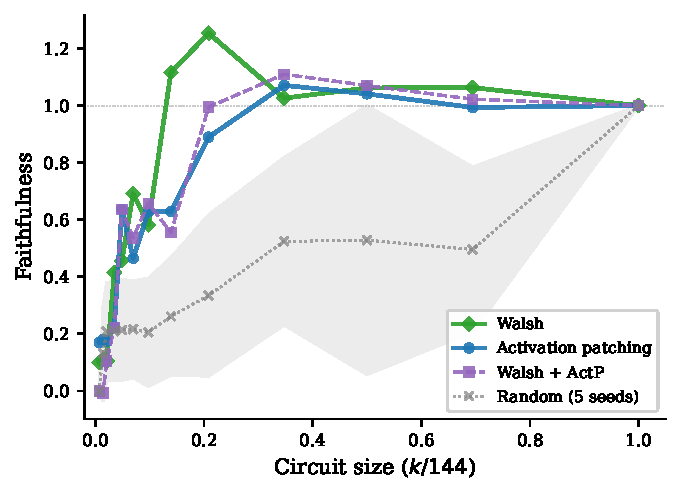
\includegraphics[width=0.7\textwidth]{figures/mib_faithfulness_curves.pdf}
\caption{Faithfulness as a function of circuit size ($k/144$) for
Walsh, activation patching, their rank-sum combination, and random
(mean $\pm$ standard deviation over 5 seeds). Walsh (green diamonds)
leads at small $k$ and reaches $f > 1$ at 20 heads; activation
patching (blue circles) converges more slowly. The gray band shows
the random baseline. All structured methods converge by $k \approx
50$ heads.}
\label{fig:mib-curves}
\end{figure}



% =====================================================================
% Draft section — the payoff section of the epistasis paper.
% Argument: the preceding sections rank discovery methods by retained
% interaction structure. This section shows what that structure contains,
% and therefore what an additive circuit discards.
%
% Status: first draft, unreviewed. Compiles clean standalone.
% Requires: booktabs, amsmath, amssymb, natbib (\citet/\citep).
% Bib entries still needed: wang2022ioi, benzer1955.
% \ref{tab:energy} points at the existing energy-fraction table — check
% the label matches before wiring this in.
% =====================================================================

\section{What the interaction structure contains}
\label{sec:what-epistasis-contains}

The preceding sections rank discovery methods by the interaction structure they retain.
That ranking earns its place only if the retained structure carries mechanism, so this
section asks what is inside the order-2 spectrum of a circuit whose mechanism is already
documented. Reading the canonical indirect object identification circuit of
\citet{wang2022ioi} against its own taxonomy recovers a dependency between two of its head
classes that the published account records as unexplained.

\subsection{Double ablation decides whether two components are one unit}

Genetics has decided whether two mutations belong to one unit or two since the 1950s, using
a test that requires no knowledge of what the unit is made of. Two recessive mutations are
placed in \emph{trans}, and the phenotype of the double heterozygote decides one locus or
two \citep{benzer1955}. The reading is a sign convention on the interaction between the two
perturbations:

\begin{center}
\begin{tabular}{lll}
\toprule
interaction & reading & verdict \\
\midrule
sub-additive (masking) & one pathway; the second hit has nothing left to break & same unit \\
additive & independent pathways & different units \\
super-additive (synergy) & parallel pathways, each covering for the other & different units \\
\bottomrule
\end{tabular}
\end{center}

An exhaustive coalition sweep supplies exactly this data for every head pair at once. For a
circuit of $n$ heads, the $2^n$ coalition values determine every order-2 Walsh coefficient
$w_{ij}$ exactly, with no regularization and no held-out set. Taking $M_{ij} = -w_{ij}$
under the convention above yields a signed masking matrix over all $\binom{n}{2}$ pairs.
Magnitude alone is uninterpretable here, since masking and synergy are both large
$|w_{ij}|$; the sign carries the verdict.

Interpretability assigns head roles from what a head appears to do. Applying the
complementation test to those roles asks whether the names track a functional criterion.

\subsection{The taxonomy separates induction and name-mover heads, and merges two others}

Hierarchical clustering on $M$ for the 15-head IOI circuit, with cluster count selected by
silhouette, recovers induction heads (L5H5, L6H9) and name-mover heads (L9H9, L10H0) as
exact units. Adjusted Rand Index against the published labels is $+0.571$ as a point
estimate, with a bootstrap-over-prompts 95\% interval of $[+0.125, +0.571]$. The taxonomy
therefore tracks interaction structure, by an amount the resampling leaves uncertain.

One boundary fails, and it fails stably. S-inhibition heads and negative name movers occupy
a single cluster in \textbf{1000 of 1000} bootstrap resamples, while the global partition
wobbles across the same draws. The merge holds in every robustness condition we ran: mean
ablation as well as zero, circuits from EAP-IG and from order-1 Walsh discovery as well as
the order-2 circuit, and complete and Ward linkage as well as average. Under a larger set of
role labels the bootstrap merge rate falls to $81$--$86\%$ on the zero-ablation conditions
and remains at $100\%$ on the others, so the pair separates occasionally once the clustering
has more classes available to it.

Depth does not explain this. Roles in IOI are layer-stratified, so a clustering that
recovered depth would score well against roles by accident. The derived partition matches
role at ARI $0.571$, raw layer at $0.053$, and layer band at $0.217$, while role itself
matches layer band at $0.526$. The clustering tracks role an order of magnitude better than
depth.

\subsection{The merge is asymmetric, and the asymmetry is the result}

Figure 2 of \citet{wang2022ioi} places name movers, negative name movers, and backup name
movers inside one group, with S-inhibition writing the queries of all three. On that
topology, removing S-inhibition disables what the group does, and a merge between
S-inhibition and any member follows.

The data merge one member and separate the other:

\begin{center}
\begin{tabular}{lc}
\toprule
class pair & merged in \\
\midrule
S-inhibition $\sim$ negative name mover & 4 / 4 conditions \\
S-inhibition $\sim$ name mover & 0 / 2 conditions \\
name mover $\sim$ negative name mover & 0 / 2 conditions \\
\bottomrule
\end{tabular}
\end{center}

\citet{wang2022ioi} state the only difference between the two classes: the negative heads
``share all the same properties as Name Mover Heads except they (1) write in the opposite
direction of names they attend to and (2) have a large negative copy score.'' Same query
source, same key and value input, same output edge, opposite OV sign. A topological account
of the merge predicts that S-inhibition masks both classes, and the circuit diagram has no
element that would distinguish them.

\subsection{The negative heads invert rather than diminish}

The OV sign difference predicts the asymmetry. Negative name movers write the negation of
whatever they attend to. With S-inhibition intact they attend to the indirect object and
write $-\mathrm{IO}$, which lowers the logit difference. Removing S-inhibition redirects
their attention to the subject, so they write $-\mathrm{S}$, which \emph{raises} the logit
difference $\mathrm{IO} - \mathrm{S}$. Their contribution inverts. Name movers copy
positively, so losing S-inhibition degrades them toward zero without changing their sign.

The exhaustive lattice tests this directly. Restricting to coalitions in which all
S-inhibition heads are retained, and separately to those in which all are removed, the
marginal contribution $\mathbb{E}_S[v(S \cup \{i\}) - v(S)]$ is exact in each condition:

\begin{center}
\begin{tabular}{llrrr}
\toprule
class & head & S-inh.\ retained & S-inh.\ removed & sign flips \\
\midrule
negative name mover & L10H7  & $-0.130$ & $+0.137$ & 1000 / 1000 \\
negative name mover & L11H10 & $-0.057$ & $+0.180$ & 1000 / 1000 \\
name mover          & L9H9   & $+0.129$ & $-0.012$ & 878 / 1000 \\
name mover          & L10H0  & $+0.149$ & $+0.009$ & 318 / 1000 \\
\bottomrule
\end{tabular}
\end{center}

Figure~\ref{fig:conditional-marginal} visualizes the pattern. Both negative heads invert in
every bootstrap draw, moving from clearly harmful to clearly helpful. The name movers decay toward zero: L10H0 keeps its sign, and L9H9 crosses zero at a
magnitude of $0.012$, which is indistinguishable from no contribution at all. Sign reversal and neutralization are distinct outcomes. They produce the two
interaction signs the clustering found: S-inhibition with negative name movers
gives $-0.267$ (masking, one unit), while S-inhibition with name movers gives
$+0.141$ (synergy, two units).

\begin{figure}[t]
\centering
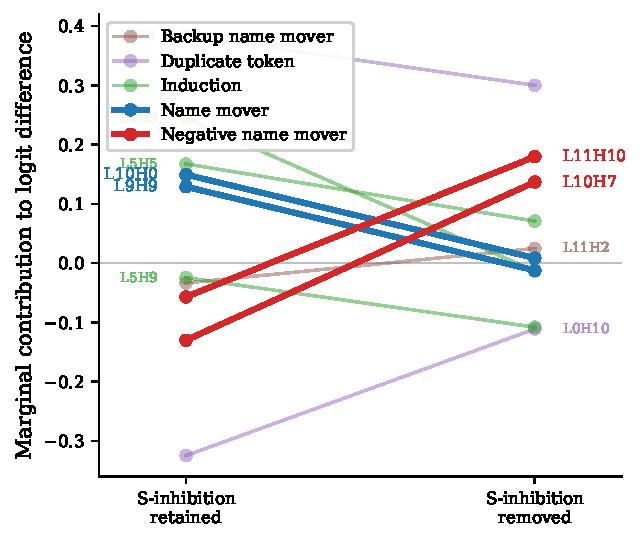
\includegraphics[width=0.65\textwidth]{figures/conditional_marginal.pdf}
\caption{Marginal contribution of each head to logit difference,
conditioned on whether S-inhibition heads are retained (left) or removed
(right). The two negative name movers (red) cross zero, inverting from
harmful to helpful. Name movers (blue) decay toward zero without
inverting. Other head classes show moderate attenuation. Bootstrap sign-flip
rates: both negative name movers flip in 1000/1000 draws.}
\label{fig:conditional-marginal}
\end{figure}

\citet{wang2022ioi} observed a fragment of this effect under a different conditioning set.
After knocking out name movers, they report that ``the Negative Name Mover Heads have a less
negative effect on logit difference, and 10.7 even has a positive effect on the logit
difference after the knockout,'' and conclude that ``[b]oth the reason and the mechanism of
this compensation effect are still unclear.'' Path patching measures one edge against a
fixed background, which makes a dependency of this kind visible only where the background
happens to expose it. The interaction decomposition holds the whole lattice, so the
dependency appears for both heads, with a magnitude and a stability attached.

\subsection{What an additive circuit discards}

This dependency lives entirely in order-2. A circuit summarized by its order-1 coefficients
retains that negative name movers lower the logit difference on average, and loses that the
sign of their contribution is set by an upstream class. The EAP-IG circuit
carries $90.4\%$ of its energy at order 1 against the canonical circuit's $78.6\%$
(Table~\ref{tab:energy}), and that gap is the room in which effects like the sign inversion sit.

\begin{table}[h]
\centering
\begin{tabular}{lccc}
\toprule
Circuit & Order 1 (\%) & Order 2 (\%) & Order 3{+} (\%) \\
\midrule
EAP-ranked           & 90.4 & 9.0  & 0.6 \\
Canonical (Wang)     & 78.6 & 18.4 & 3.0 \\
Walsh-ranked         & 80.9 & 16.8 & 2.3 \\
Epistasis-ranked     & 78.4 & 18.6 & 3.0 \\
Random               & 97.9 & 2.1  & 0.0 \\
\bottomrule
\end{tabular}
\caption{Fraction of nonconstant Walsh energy at each interaction order
for five 15-head IOI circuits under mean ablation. The EAP-ranked circuit
concentrates energy at order 1; circuits selected for functional relevance
(canonical, Walsh, epistasis) retain 17--19\% at order 2.}
\label{tab:energy}
\end{table}

The consequence for practice is narrow and concrete. A head's measured contribution is a
property of the head together with the background it was measured against, and reporting it
as a property of the head alone is safe only when the order-2 terms coupling it to the rest
of the circuit are small. Those terms are measurable, so the assumption is checkable rather
than assumed.

% ---------------------------------------------------------------------
% NOTES FOR REVISION
%
% 1. Figure to make: conditional marginal contribution for all labelled
%    heads, S-inh retained vs removed, as a slope chart. The two negative
%    heads cross zero in opposite direction to everything else — that is
%    the whole result in one image. Data: results/v13_conditional_marginal.json
%
% 2. Scope sentence still owed somewhere in this section or in limitations:
%    one model (GPT-2 small), one task (IOI), merge rests on five heads,
%    sign-flip result on two. Whether sign inversion generalizes to other
%    inhibitory pairings is untested.
%
% 3. Provenance sentence owed in methods: the complementation analysis was
%    preregistered (prereg_v13, sha 1f915bbc, amended e258d592); the
%    conditional-marginal test in 4.4 was derived from the pairwise result
%    and is a follow-up rather than a registered prediction. One sentence,
%    methods only.
%
% 4. The ARI numbers here are from the registered 10-label analysis. A later
%    run with an expanded 18-label dictionary gives lower ARIs (0.106-0.290,
%    one negative). Do not mix the two sets in one table. The merge holds
%    under both; only the merge should be quoted across label sets.
%
% 5. Table \ref{tab:energy} is the existing energy-fraction table from the
%    results section; check the label matches before compiling.
% ---------------------------------------------------------------------


% =====================================================================
% Discussion — selective pressures and implications.
%
% Status: v1 first draft. Compiles with main.tex.
% =====================================================================

\section{Discussion}
\label{sec:discussion}

\subsection{The selective-pressure analogy}

Circuit discovery methods are evaluation instruments, and every
instrument selects for what it measures. Activation patching selects for
heads whose individual removal changes the target metric. EAP selects
for edges along which gradients flow. Path patching selects for direct
causal influence through the residual stream. Each method returns a
``circuit'' that is faithful to the full model, but the circuits differ
in which interaction structure they preserve.

The Walsh--Hadamard decomposition provides a fixed reference frame for
quantifying these differences. The interaction spectrum of a circuit on
a task is a property of the model, independent of how the circuit was
discovered. Two methods that return the same circuit preserve the same
spectrum; two methods whose head rankings correlate at $\rho = 0.58$
(EAP) versus $\rho = 0.07$ (path patching) preserve detectably
different structure. The ``right'' discovery method depends on what
the analyst wants to learn: marginal importance, direct wiring, or
functional coupling.

\subsection{Implications for circuit interpretation}

The complementation test in
Section~\ref{sec:what-epistasis-contains} shows that interaction
structure carries mechanism. The sign inversion of negative name movers
is invisible to any method that reports only marginal importance: the
head's average contribution is negative, and its contribution
conditional on the state of upstream S-inhibition heads flips sign
entirely. Reporting the head's marginal score as its property elides
the dependency that determines whether the head helps or hurts.

This is a general warning, not specific to IOI. A head whose
contribution depends on the state of another head is the rule rather
than the exception whenever order-2 energy exceeds a few percent of
the total spectrum. The fraction of energy at each order is measurable
from the Walsh spectrum, so the severity of the problem is quantifiable
for any circuit.

\subsection{Limitations}

\paragraph{One model, one task.}

All results use GPT-2 small on IOI. The Walsh--Hadamard transform
applies to any model and task where components can be ablated and a
scalar metric computed, but the empirical findings --- the correlation
between Walsh and EAP, the orthogonality of Walsh and path patching,
the complementation-test result --- may not generalize. The compressed
sensing protocol makes it feasible to run the same analysis on larger
models and different tasks.

\paragraph{Heads only.}

The current decomposition treats attention heads as the atomic
components. MLPs, individual neurons, and attention positions are
excluded. Extending to finer granularity increases $n$ and the number
of target coefficients, but the compressed sensing approach scales
as $O(k \log k \log N)$, not $O(2^n)$, so moderate increases are
tractable.

\paragraph{Ablation dependence.}

The Walsh spectrum depends on the ablation primitive
(Section~\ref{sec:weight-geometry}). Mean and resample ablation agree
moderately ($\gamma = 0.43$); zero ablation agrees with neither
($\gamma = 0.14$). The interaction structure is not a unique property
of the circuit --- it is a property of the circuit together with the
measurement method. This parallels the situation in quantitative
genetics, where different loss-of-function assays yield different
interaction
estimates~\citep{housden2017comparison,fluidity2024elife}.

\paragraph{Faithfulness metric choice.}

MIB faithfulness (Section~\ref{sec:mib-benchmark}) measures how well a
circuit reproduces the full model's logit difference under mean ablation.
\citet{chughtai2024faithfulness} show that faithfulness metrics are not
robust to the choice of ablation primitive or metric. Our results should
be interpreted as specific to mean ablation on logit difference, not as
general claims about circuit quality.

\subsection{Future directions}

The sparse Walsh recovery protocol converts interaction analysis from a
small-circuit diagnostic into a practical method applicable wherever
activation patching can identify a candidate head set. Running the
analysis on multiple models (GPT-2 medium, Pythia, Llama) and tasks
(greater-than, gendered pronoun resolution) would test whether the
selective-pressure pattern generalizes. Extending the decomposition to
MLP neurons alongside attention heads would capture cross-component
interactions that the head-only analysis misses. Combining Walsh
interaction rankings with EAP edge scores --- rather than with path
patching, which measures an orthogonal quantity --- may produce circuits
that are both faithful and interaction-preserving.


% ------------------------------------------------------------------
\bibliographystyle{tmlr}
\bibliography{references}

\end{document}
